\subsection{Zylinderresonator}
\subsubsection{Schallgeschwindigkeit}
Mittels der Gleichung \eqref{eq:resonanz} lässt sich für die Daten aus Tabelle \ref{tab:zylinder} ein Fit der der Form
\begin{equation}
  \Delta f = \frac{c}{2L}
\end{equation}
herleiten. Dieser wird mit der curve\_fit Funktion von scipy \cite{scipy} gefittet und ergibt die Schallgeschwindigkeit
\begin{equation}
  c_{Messung} =(339,33\pm 0,54)\si{\metre\per\second}.
\end{equation}
und den Graphen in Abbildung \ref{fig:plot_zylinder}.
Dieser Wert liegt nahe an einem Theoriewert \cite{schall} für Raumtemperatur ($20°$C) und normalem Atmosphärendruck (Beides konnte nicht gemessen werden und wird daher angenommen).
\begin{equation}
  c_{Theorie} =343\si{\metre\per\second}
\end{equation}


\begin{figure}
  \centering
  \includegraphics{build/plot.pdf}
  \caption{Frequenzdifferenz in Abhängigkeit der Länge eines Zylinderresonators}
  \label{fig:plot_zylinder}
\end{figure}

\subsubsection{Resonanzsweep in Zylinderketten}
Der durchgeführte Resonanzsweep (1-10 kHz) zeigt ähnliche Ergebnisse beim Oszilloskop und PC, wie in Abbildung \ref{fig:plot_2zylinder_sweep} zu erkennen ist.
Die Bilder des PC's sind aber von deutlich besserer Qualität, weshalb diese bei allen weiteren Messungen zur Auswertung verwendet werden.
Die, in den Abbildungen \ref{fig:plot_2zylinder_sweep} und \ref{fig:plot_zylinder_sweep} dargestellten, Resonanzsweeps bestätigen die Resonanzbedingung \eqref{eq:resonanz} aus der Theorie durch ihre stetig ansteigende Anzahl an Resonanzpeaks.
\begin{figure}
  \centering
  \begin{subfigure}{0.48\textwidth}
    \centering
    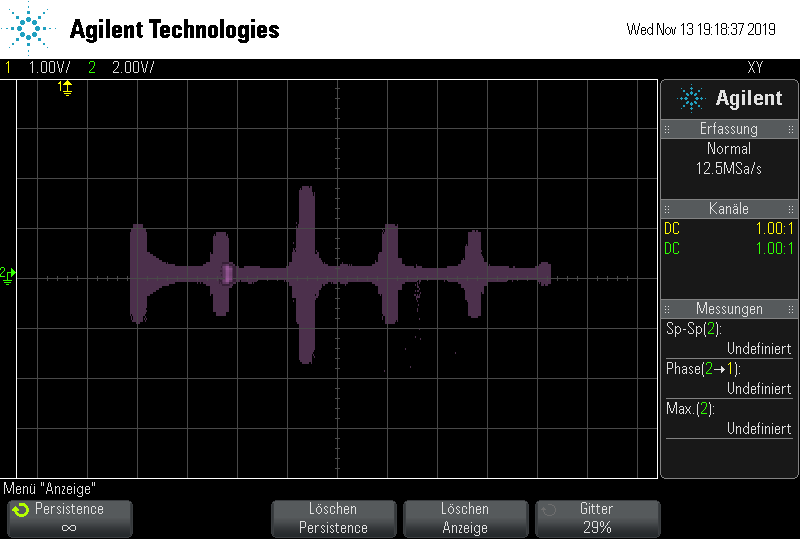
\includegraphics[width=0.9\textwidth]{Bilder/Oszillator_Zylindermessung/scope_0.png}
    \caption{Am Oszilloskop}
  \end{subfigure}
  \begin{subfigure}{0.48\textwidth}
    \centering
    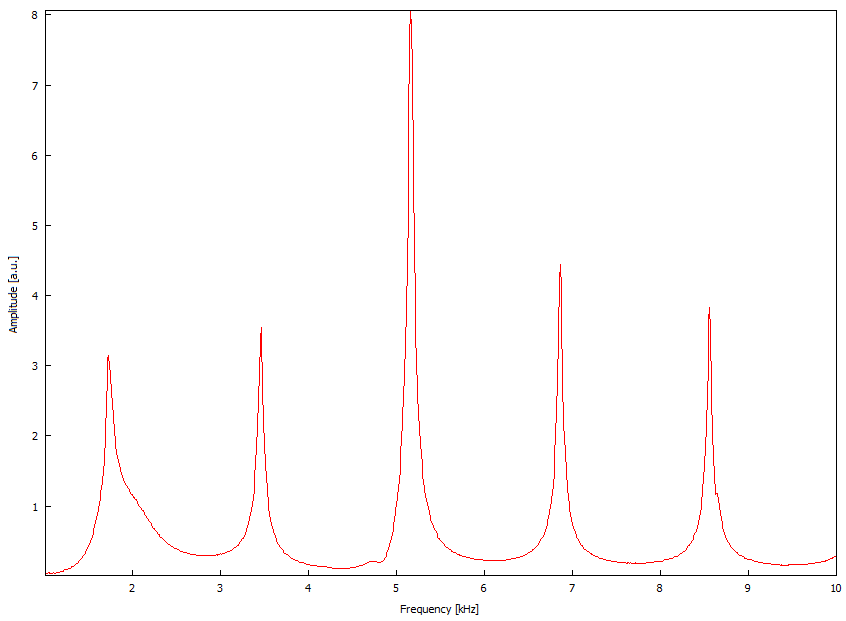
\includegraphics[width=0.9\textwidth]{Bilder/PC_Zylindermessung/2_Zylinder.png}
    \caption{Am PC}
  \end{subfigure}
  \caption{Resonanzsweep bei 2 50mm Zylindern am Oszilloskop und am PC}
  \label{fig:plot_2zylinder_sweep}
\end{figure}

\begin{figure}
  \centering
  \begin{subfigure}{0.32\textwidth}
    \centering
    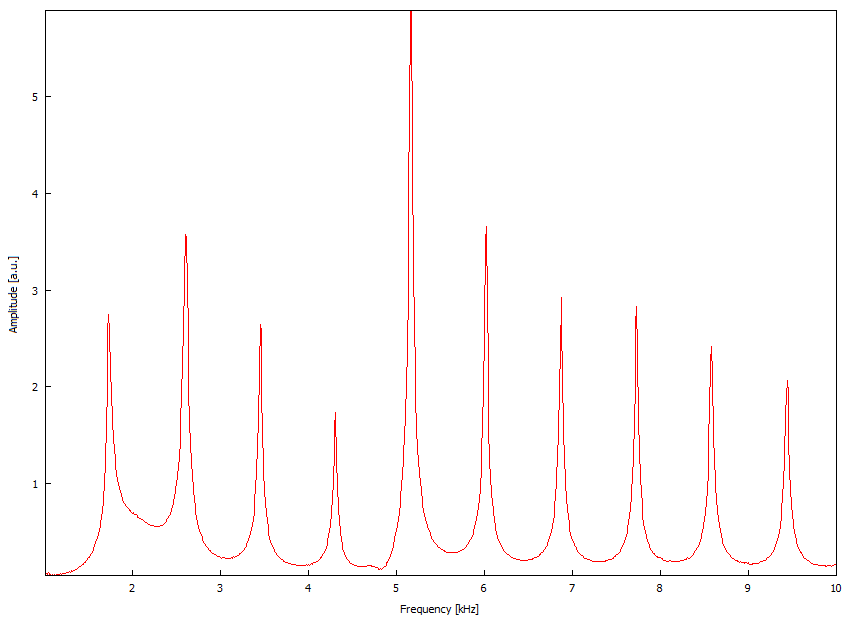
\includegraphics[width=0.9\textwidth]{Bilder/PC_Zylindermessung/4_Zylinder.png}
    \caption{4 Zylinder}
  \end{subfigure}
  \begin{subfigure}{0.32\textwidth}
    \centering
    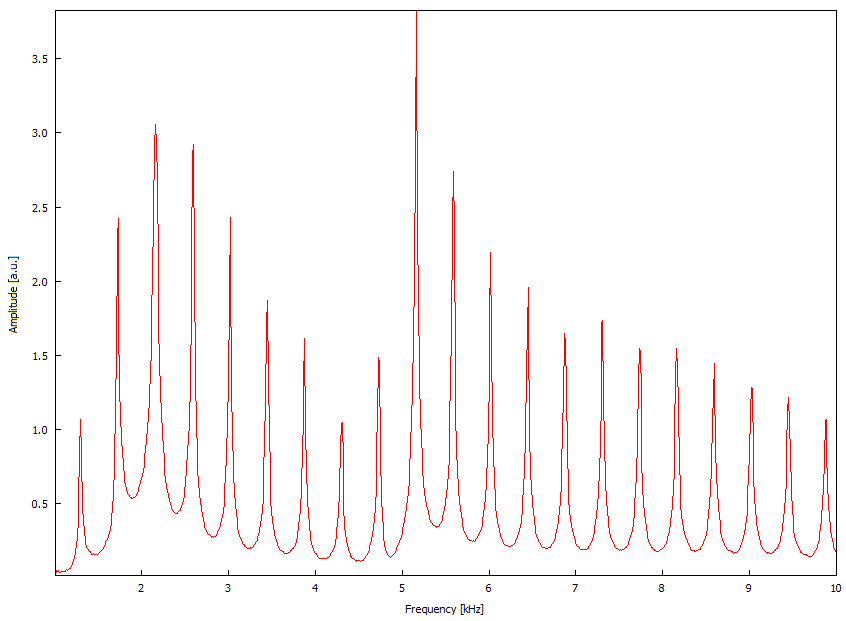
\includegraphics[width=0.9\textwidth]{Bilder/PC_Zylindermessung/8_Zylinder.png}
    \caption{8 Zylinder}
  \end{subfigure}
  \begin{subfigure}{0.32\textwidth}
    \centering
    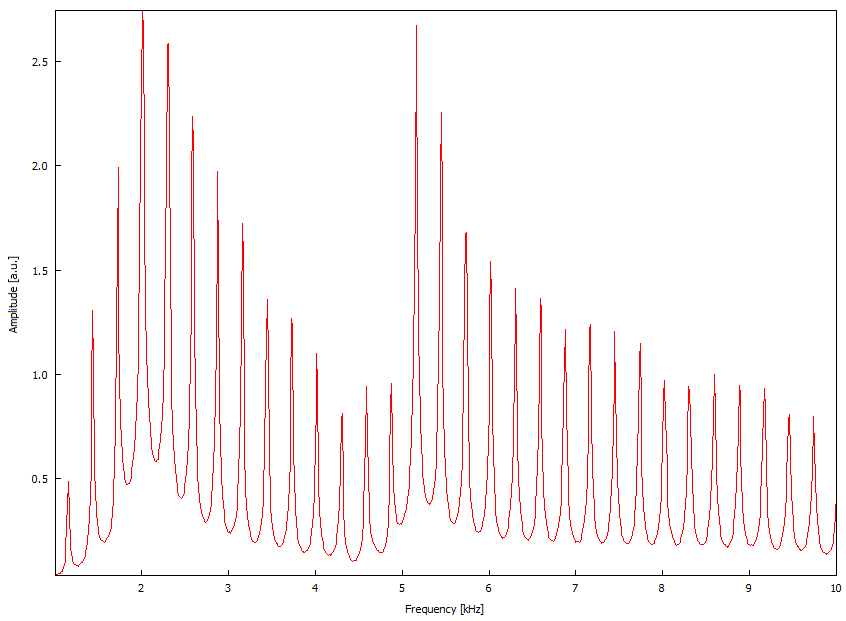
\includegraphics[width=0.9\textwidth]{Bilder/PC_Zylindermessung/12_Zylinder.png}
    \caption{12 Zylinder}
  \end{subfigure}
  \caption{Resonanzsweep von mehreren 50mm Zylindern am PC}
  \label{fig:plot_zylinder_sweep}
\end{figure}

\subsection{Kugelresonator}
\subsubsection{Resonanzfrequenzen}
Die mit dem Oszilloskop aufgenommenen Resonanzfrequenzen stehen in Tabelle \ref{tab:kugel_resonanz}.
Der im gleichen Bereich aufgenommene Frequenzsweep mit dem PC aus Abbildung \ref{fig:kugel_resonanz} weist ein paar mehr Peaks auf,
die aber relativ nahe an anderen Peaks liegen und dadurch nicht mit dem Oszilloskop aufgelöst werden konnten.

\begin{figure}
  \centering
  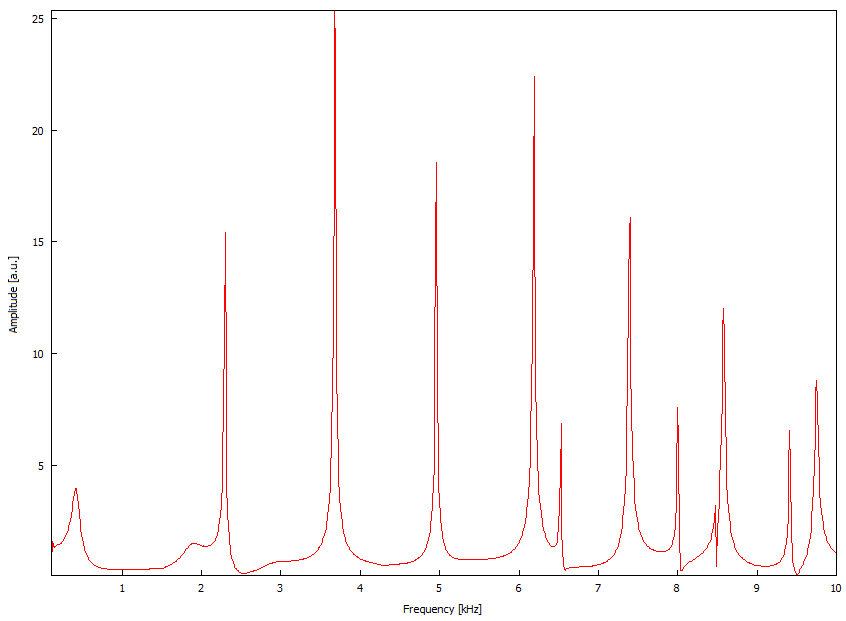
\includegraphics[width=0.8\textwidth]{Bilder/PC_Kugelresonator/180_100-10000Hz.png}
  \caption{Resonanzspektrum des Kugelresonators bei 100-10000Hz}
  \label{fig:kugel_resonanz}
\end{figure}

\subsubsection{Winkelabhängigkeit}
Da unser Messwinkel $\alpha$ nicht senkrecht zur Symmetrieachse liegt, muss dieser umgeformt werden können um ihn in die Kugelflächenfunktionen einzusetzen.
Die Beziehung erfolgt aus trigonometrischen Überlegungen und ergibt sich als 
\begin{align}
  \cos(\theta)&=\frac{1}{2}\left(\cos(\alpha)-1\right)\nonumber\\
  \theta&=\arccos\left(\frac{1}{2} \left(\cos(\alpha)-1\right)\right).\label{eq:alpha_zu_theta}
\end{align}
Die ersten Kugelflächenfunktionen (normiert nach max$(Y)=1$) ergeben sich als
\begin{align}
  Y_{00} &= 1\\
  Y_{10} &= \text{cos}(\theta)\\
  Y_{20} &= \frac{1}{2}(3\text{cos}^2(\theta)-1) \\
  Y_{30} &= \frac{1}{2}(5\text{cos}^3(\theta)-3\text{cos}(\theta))\\
  Y_{40} &= \frac{1}{8}(35\text{cos}^4(\theta)-30\text{cos}^2(\theta)+3)\\
  Y_{50} &= \frac{1}{8}(\text{cos}(\theta)\cdot(63\text{cos}^4(\theta)-70\text{cos}^2(\theta)+15))
\end{align}
Werden nun die Daten aus Tabelle \ref{tab:kugel_resonanz_winkel} nach Gleichung \eqref{eq:alpha_zu_theta} umgeformt, ebenfalls nach max$(A)=1$ normiert
und in einem Polarplot geplottet, ergeben sich die Plots aus Abbildung \ref{fig:kugel_resonanz_winkel}.
Die zugeordeneten Kugelflächenfunktionen sind hierbei per Auge gewählt worden und haben aufgrund der Normierung keine Fit-Parameter.

\begin{figure}
  \centering
  \begin{subfigure}{0.32\textwidth}
    \centering
    \includegraphics[width=\textwidth]{build/Kugel_Winkel_3.pdf}
    \caption{$3,666$kHz}
  \end{subfigure}
  \begin{subfigure}{0.32\textwidth}
    \centering
    \includegraphics[width=\textwidth]{build/Kugel_Winkel_6.pdf}
    \caption{$6,174$kHz}
  \end{subfigure}
  \begin{subfigure}{0.32\textwidth}
    \centering
    \includegraphics[width=\textwidth]{build/Kugel_Winkel_7.pdf}
    \caption{$7,379$kHz}
  \end{subfigure}
  \caption{Normierte Amplituden in Abhängigkeit vom Winkel \theta}
  \label{fig:kugel_resonanz_winkel}
\end{figure}

\subsubsection{Peakaufspaltung}
Durch Einsetzen eines Ring in den Ring Kugelresonator entsteht eine Vorzugsrichtung und die Entartung in m wird aufgehoben.
In Abbildung \ref{fig:kugel_ringe} ist dies durch ein Aufspaltung des Peaks bei $2,3$kHz erkennen.
Die Aufspaltung wird breiter je dicker der Ring zwischen den Kugelhälften ist.
\begin{figure}
  \centering
  \begin{subfigure}{0.4\textwidth}
    \centering
    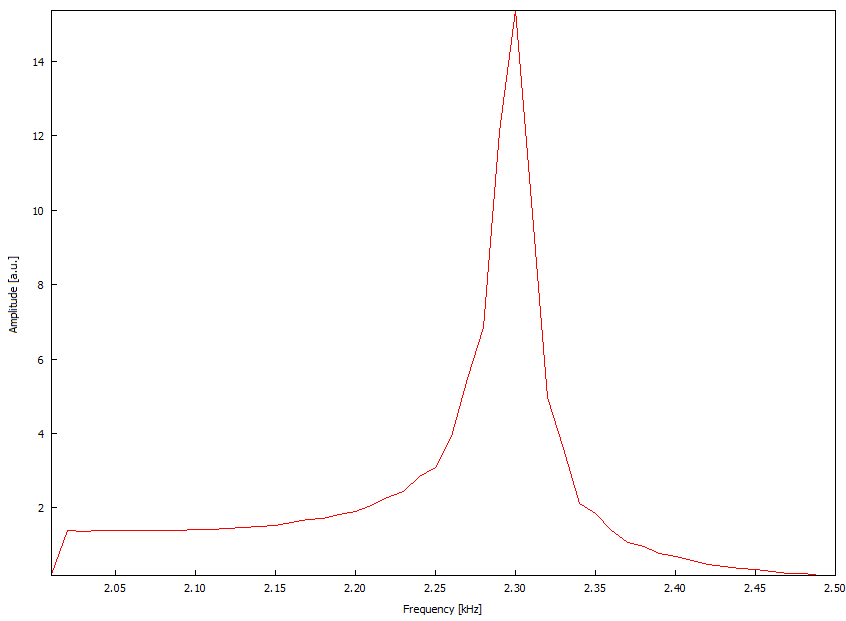
\includegraphics[width=\textwidth]{Bilder/PC_Kugelresonator/180_2000-2500_ohneRing.png}
    \caption{Ohne Ring}
  \end{subfigure}
  \begin{subfigure}{0.4\textwidth}
    \centering
    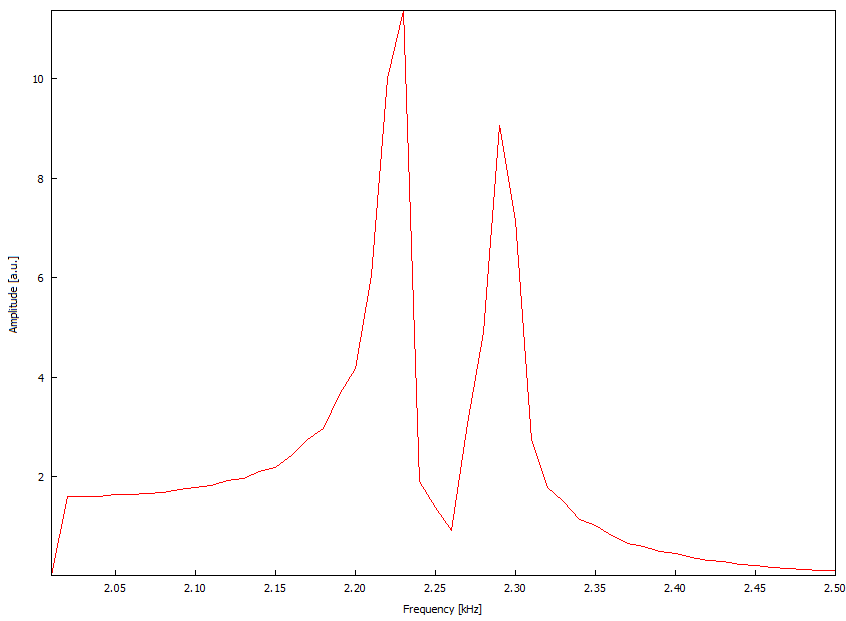
\includegraphics[width=\textwidth]{Bilder/PC_Kugelresonator/180_2000-2500_3mmRing.png}
    \caption{3mm Ring}
  \end{subfigure}
  \begin{subfigure}{0.4\textwidth}
    \centering
    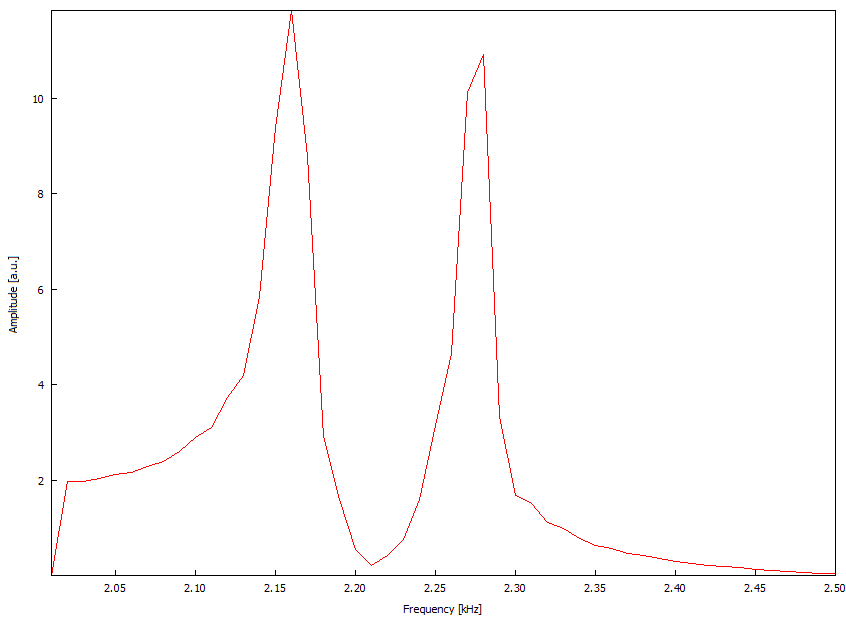
\includegraphics[width=\textwidth]{Bilder/PC_Kugelresonator/180_2000-2500_9mmRing.png}
    \caption{9mm Ring}
  \end{subfigure}
  \begin{subfigure}{0.4\textwidth}
    \centering
    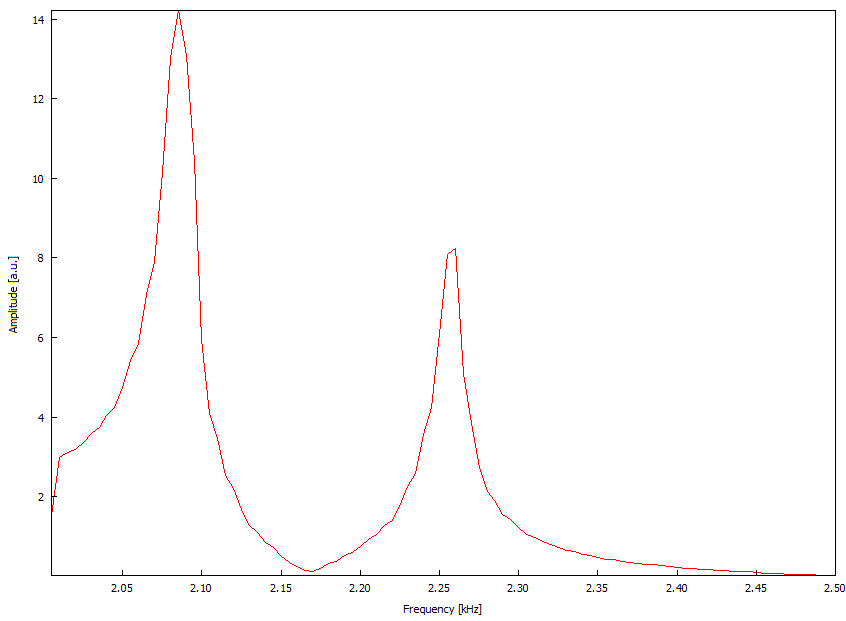
\includegraphics[width=\textwidth]{Bilder/PC_Kugelresonator/180_2000-2500_12mmRing.png}
    \caption{12mm Ring}
  \end{subfigure}
  \caption{Aufspaltung des Resonanzpeaks bei $2,3$kHz}
  \label{fig:kugel_ringe}
\end{figure}

Mit der Messung aus Tabelle \ref{tab:kugel_ring} lassen sich die Abbildungen \ref{fig:kugel_ring} erstellen.
Es ist zu beachten, dass durch die Vorzugsrichtung nur $\phi$ gemessen wurde.
Die $\phi$-Abhängigkeit der Kugelflächenfunktionen ergibt sich als
\begin{equation}
  Y_m \sim e^{im\phi}
\end{equation}
Aus der vorherigen Messung ist $l=2$ bekannt.
Die Resonanz bei $2,146$kHz lässt sich der Funktion $Y_{20}$ zuordnen und die Resonanz bei $2,257$kHz  der Funktion $Y_{21}$.
\begin{figure}
  \centering
  \begin{subfigure}{0.4\textwidth}
    \centering
    \includegraphics[width=\textwidth]{build/Kugel_Ring_21.pdf}
    \caption{$2,146$kHz}
  \end{subfigure}
  \begin{subfigure}{0.4\textwidth}
    \centering
    \includegraphics[width=\textwidth]{build/Kugel_Ring_22.pdf}
    \caption{$2,257$kHz}
  \end{subfigure}
  \caption{Winkelverteilung bei dem aufgespaltenem Peak um $2,2$kHz}
  \label{fig:kugel_ring}
\end{figure}

\subsection{Gekoppelte Kugelresonatoren}
Wie in den Abbildungen \ref{fig:molekül_plots} zu erkennen, bleiben die Resonanzfrequenzen um $2,3$kHz zunächst bestehen,
werden aber mehr und mehr Blenden zwischen die zwei Kugelresonatoren gelegt, wird der zweite Peak stark abgeschwächt.
Zudem wird der Peak hinter $2,4$kHz mit mehr Blenden näher an den $2,3$kHz Peak heranbewegt.
Mit den Daten aus Tabelle \ref{tab:molekül} lassen sich Plots aus Abbildung \ref{fig:molekül_plots_} erstellen.
Es ist ersichtlich, dass beiden Resonanzfrequenzen die $Y_{00}$ Mode zugewiesen werden kann.

\begin{figure}
  \centering
  \begin{subfigure}{0.4\textwidth}
    \centering
    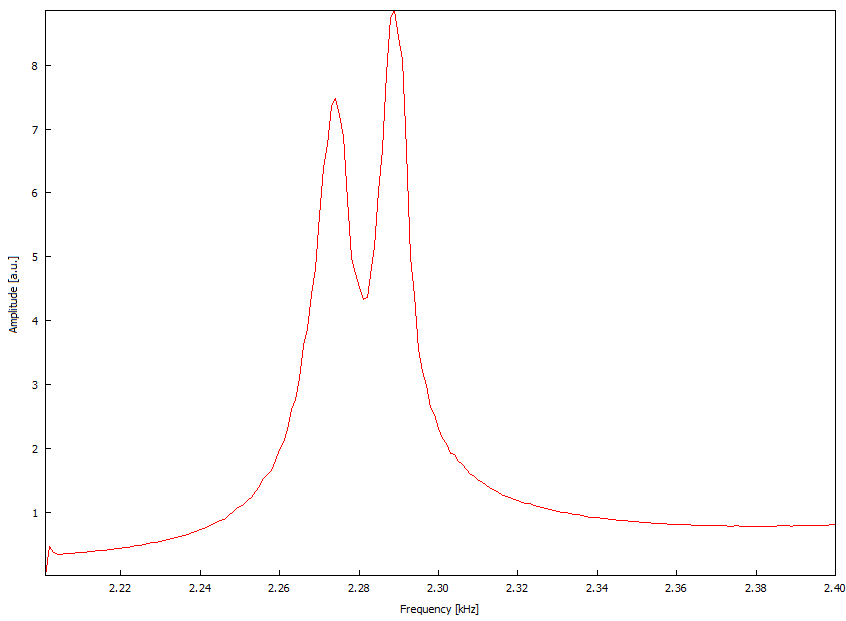
\includegraphics[width=\textwidth]{Bilder/PC_Molekül/ohne_Blende.png}
    \caption{Ohne Blende}
  \end{subfigure}
  \begin{subfigure}{0.4\textwidth}
    \centering
    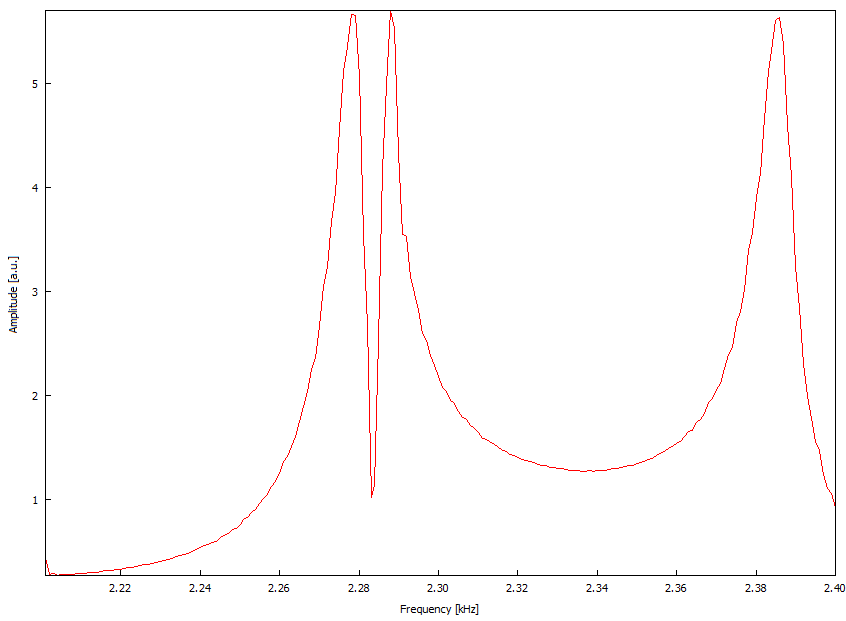
\includegraphics[width=\textwidth]{Bilder/PC_Molekül/5mm_Blende.png}
    \caption{5mm Blende}
  \end{subfigure}
  \begin{subfigure}{0.4\textwidth}
    \centering
    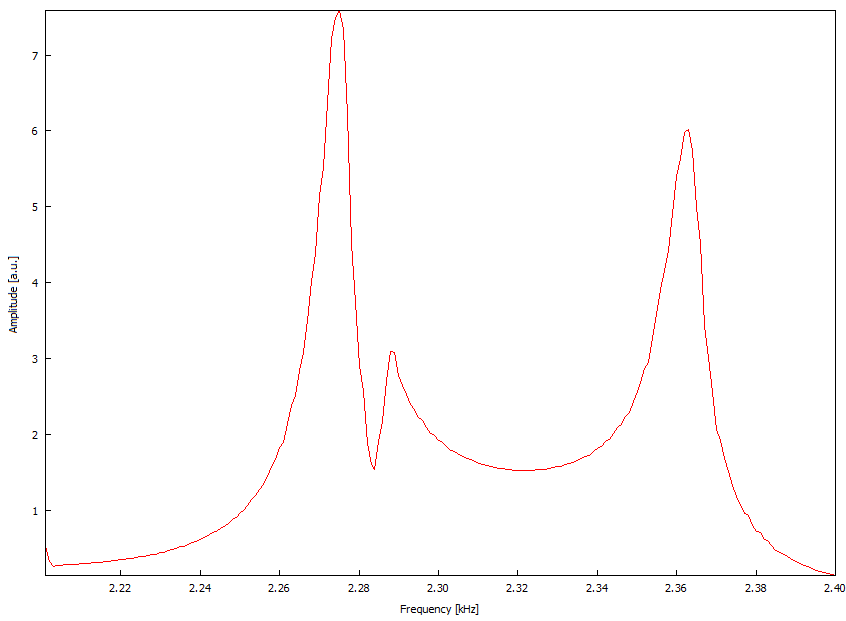
\includegraphics[width=\textwidth]{Bilder/PC_Molekül/10mm_Blende.png}
    \caption{10mm Blende}
  \end{subfigure}
  \begin{subfigure}{0.4\textwidth}
    \centering
    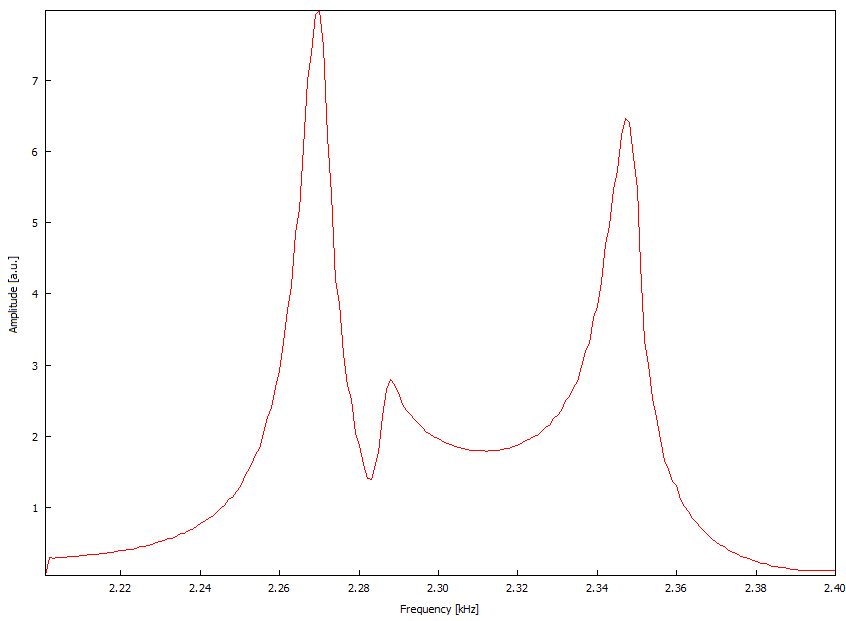
\includegraphics[width=\textwidth]{Bilder/PC_Molekül/15mm_Blende.png}
    \caption{15mm Blende}
  \end{subfigure}
  \begin{subfigure}{0.4\textwidth}
    \centering
    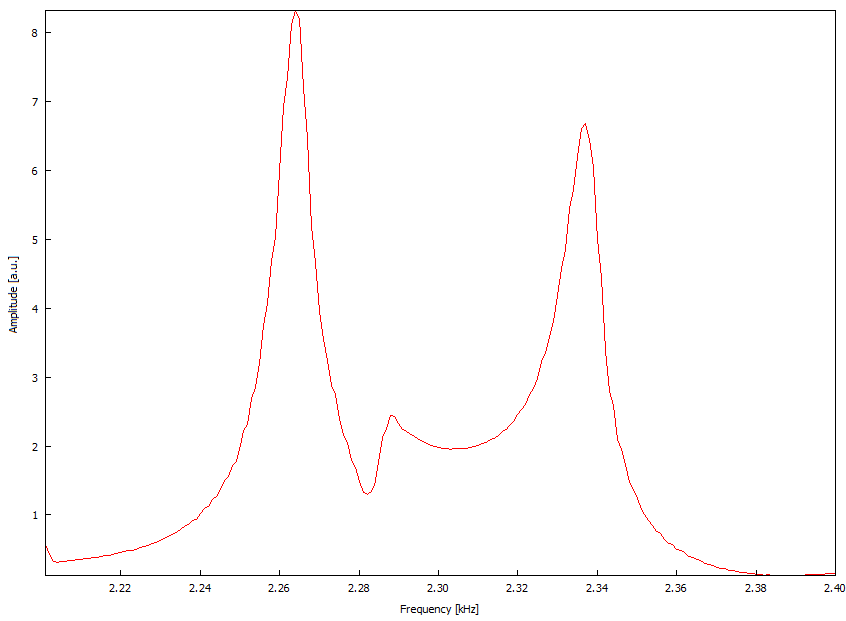
\includegraphics[width=\textwidth]{Bilder/PC_Molekül/20mm_Blende.png}
    \caption{20mm Blende}
  \end{subfigure}
  \begin{subfigure}{0.4\textwidth}
    \centering
    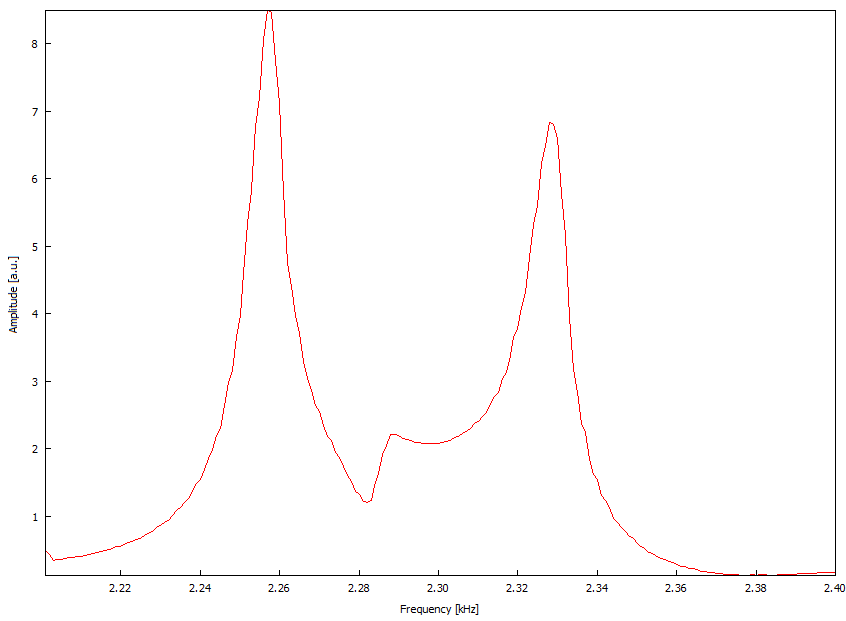
\includegraphics[width=\textwidth]{Bilder/PC_Molekül/25mm_Blende.png}
    \caption{25mm Blende}
  \end{subfigure}
  \caption{Winkelverteilung bei dem aufgespaltenem Peak um $2,2$kHz}
  \label{fig:molekül_plots}
\end{figure}

\begin{figure}
  \centering
  \begin{subfigure}{0.4\textwidth}
    \centering
    \includegraphics[width=\textwidth]{build/Molekül_Ring_22.pdf}
    \caption{$2,256$kHz}
  \end{subfigure}
  \begin{subfigure}{0.4\textwidth}
    \centering
    \includegraphics[width=\textwidth]{build/Molekül_Ring_23.pdf}
    \caption{$2,327$kHz}
  \end{subfigure}
  \caption{Winkelverteilung bei dem aufgespaltenem Peak um $2,3$kHz beim gekoppelten Resonator mit 5mm Blende}
  \label{fig:molekül_plots_}
\end{figure}

\subsection{Zylinderketten mit Blenden}
\subsubsection{Reine Ketten}
Wie an Abbildung \ref{fig:zylinder_blenden_rein} zu erkennen bilden sich mit zunehmender Zylinderzahl Resonanzbänder aus.
Es entstehen pro hinzugefügtem Zylinder eine neue Resonanzfrequenz pro Resonanzband, die Bänder werden breiter und die Bandlücken kleiner.
Es nähert sich also das System einem Sytem ohne Blenden an.

\begin{figure}
  \centering
  \begin{subfigure}{0.4\textwidth}
    \centering
    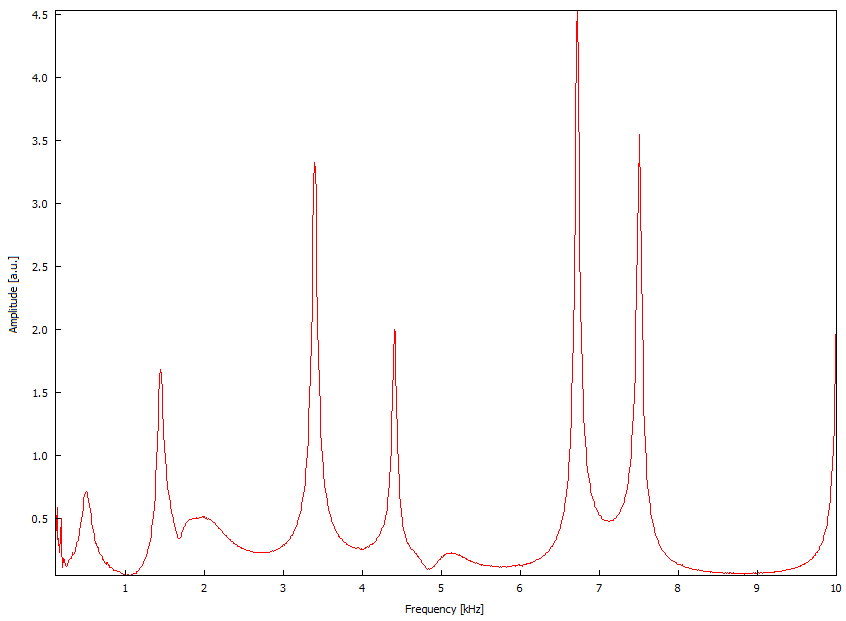
\includegraphics[width=\textwidth]{Bilder/Zylinderketten/rein_2.png}
    \caption{Zwei Zylinder}
  \end{subfigure}
  \begin{subfigure}{0.4\textwidth}
    \centering
    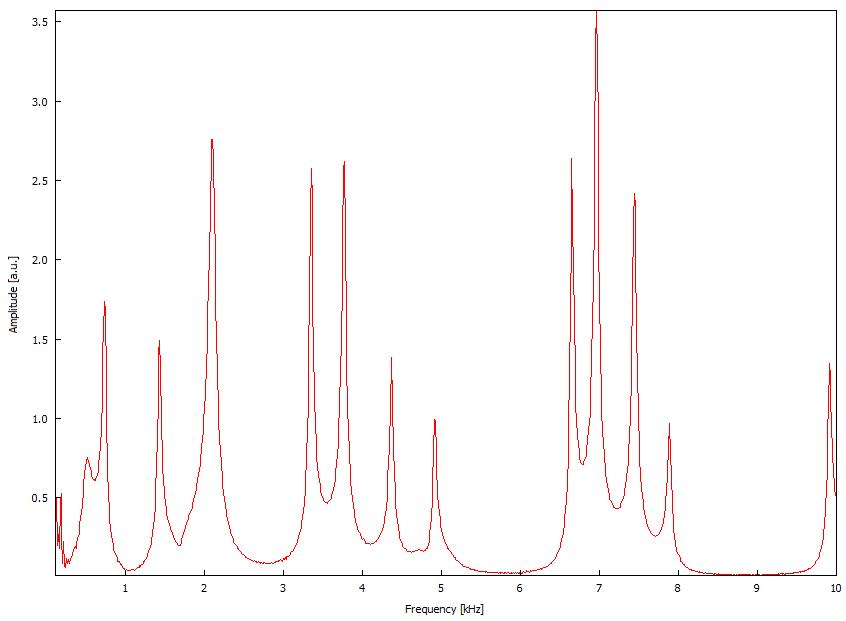
\includegraphics[width=\textwidth]{Bilder/Zylinderketten/rein_4.png}
    \caption{Vier Zylinder}
  \end{subfigure}
  \begin{subfigure}{0.4\textwidth}
    \centering
    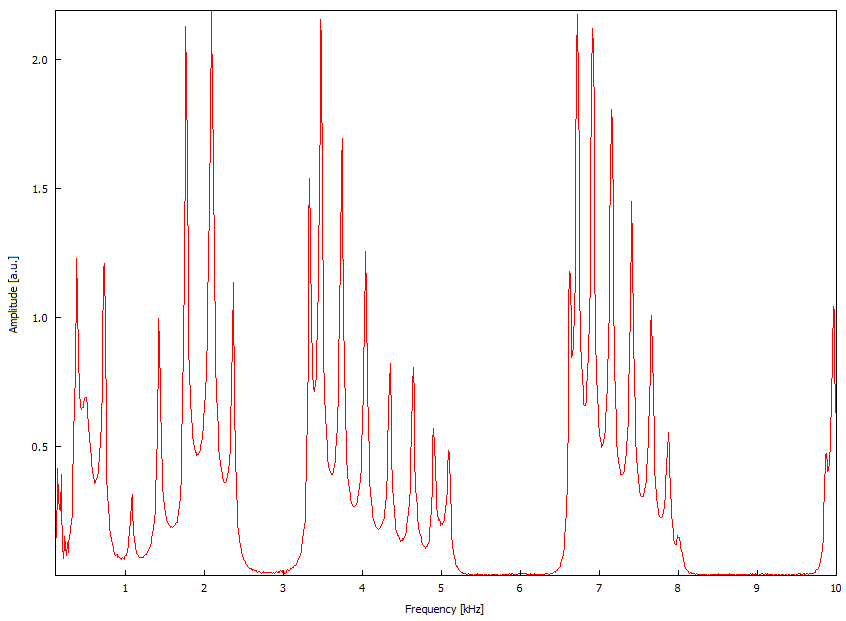
\includegraphics[width=\textwidth]{Bilder/Zylinderketten/rein_8.png}
    \caption{Acht Zylinder}
  \end{subfigure}
  \begin{subfigure}{0.4\textwidth}
    \centering
    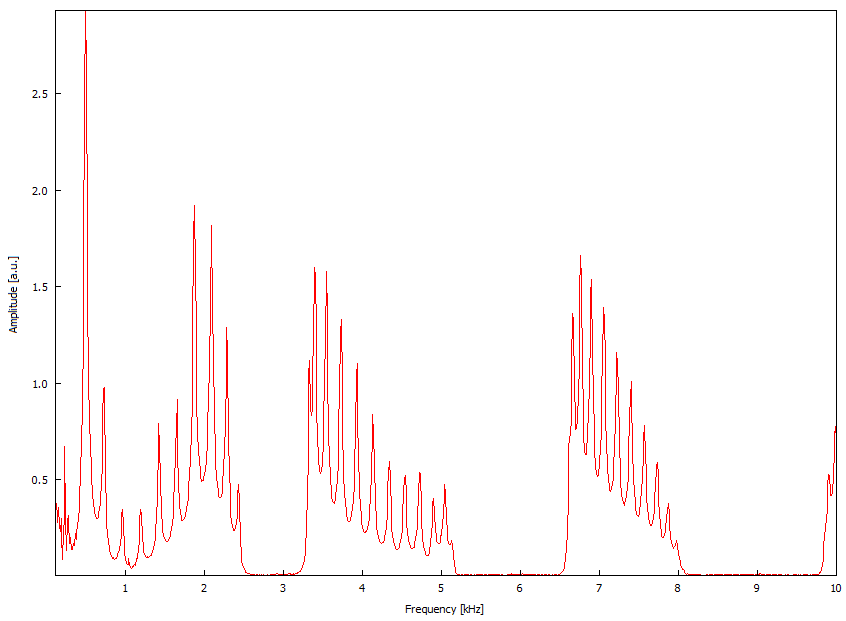
\includegraphics[width=\textwidth]{Bilder/Zylinderketten/rein_12.png}
    \caption{Zwölf Zylinder}
  \end{subfigure}
  \caption{Resonanzsweeps von Zylinderketten mit Blenden}
  \label{fig:zylinder_blenden_rein}
\end{figure}

\subsubsection{Alternierende Kette}
Der Resonanzsweep (Abbildung \ref{fig:zylinder_alternierend}) mit alternierenden Blenden sorgen für eine Aufspaltung der Resonanzbänder.
\begin{figure}
  \centering
  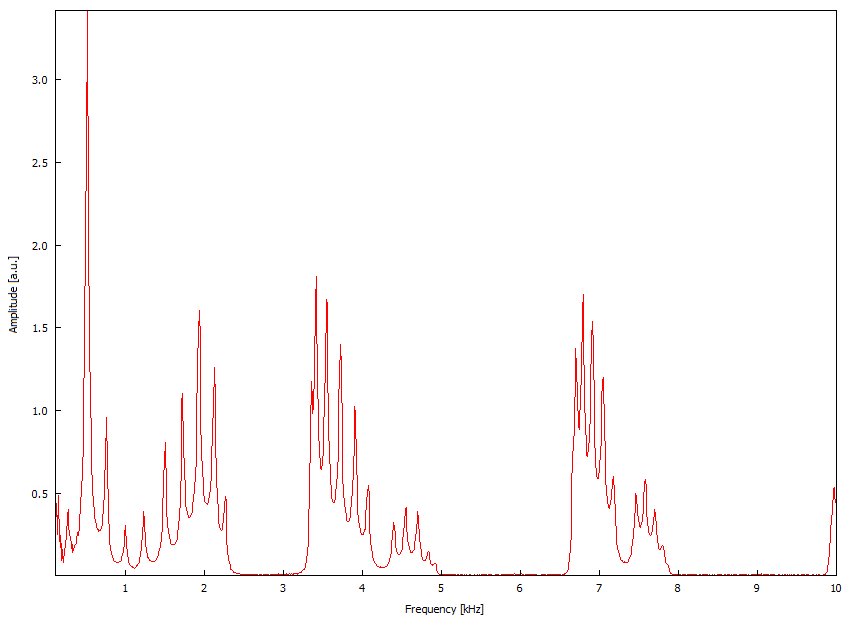
\includegraphics[width=\textwidth]{Bilder/Zylinderketten/rein_12_alternierendeBlende.png}
  \caption{Resonanzsweep einer Zylinderkette mit zwölf 50mm Zylindern und alternierenden Blenden}
  \label{fig:zylinder_alternierend}
\end{figure}

\subsubsection{Fehlstellen}
Wird der mittlere Zylinder durch einen Zylinder anderer Länge ersetzt, ergeben sich die Frequenzspektren in Abbildung \ref{fig:zylinder_fehlstellen}.
Die Resonanzbänder bleiben zwar bestehen, aber werden durch die Fehlstelle verzerrt und die individuellen Peaks werden schwieriger aufzulösen.
Es werden ausserdem neue Zustände zwischen den Bändern sichtbar.
Anders als bei den alternierenden Blenden, bei welchen sich ganze Bandstrukuren einfügten, beläuft es sich hier nur auf einzelne Zustände.
Bei der 75mm Fehlstelle ist der Effekt nicht ganz so dramatisch wie bei der $12,5$mm Fehlstelle.
\begin{figure}
  \centering
  \begin{subfigure}{0.4\textwidth}
    \centering
    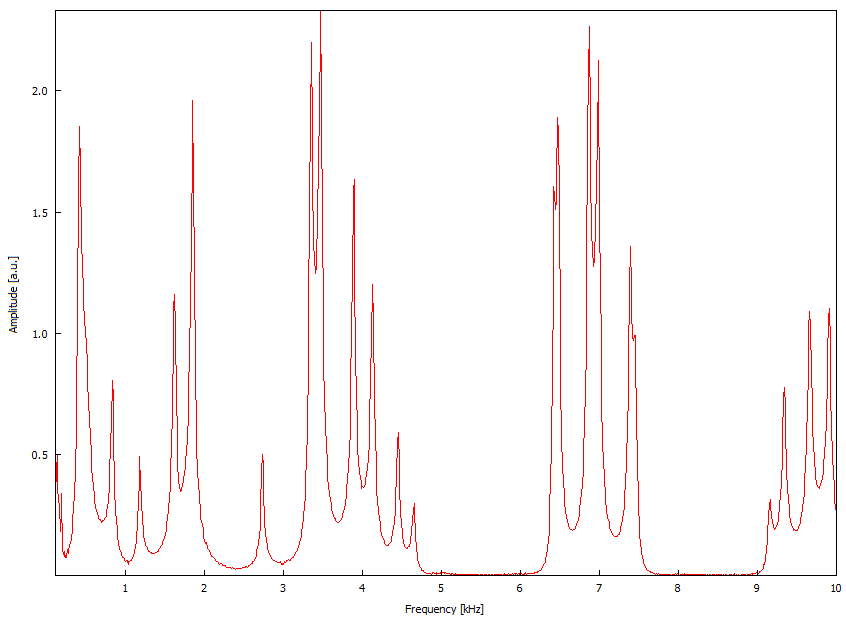
\includegraphics[width=\textwidth]{Bilder/Zylinderketten/unrein_12,5mm_mitte_doppel.png}
    \caption{$12,5$mm Fehlstelle}
  \end{subfigure}
  \begin{subfigure}{0.4\textwidth}
    \centering
    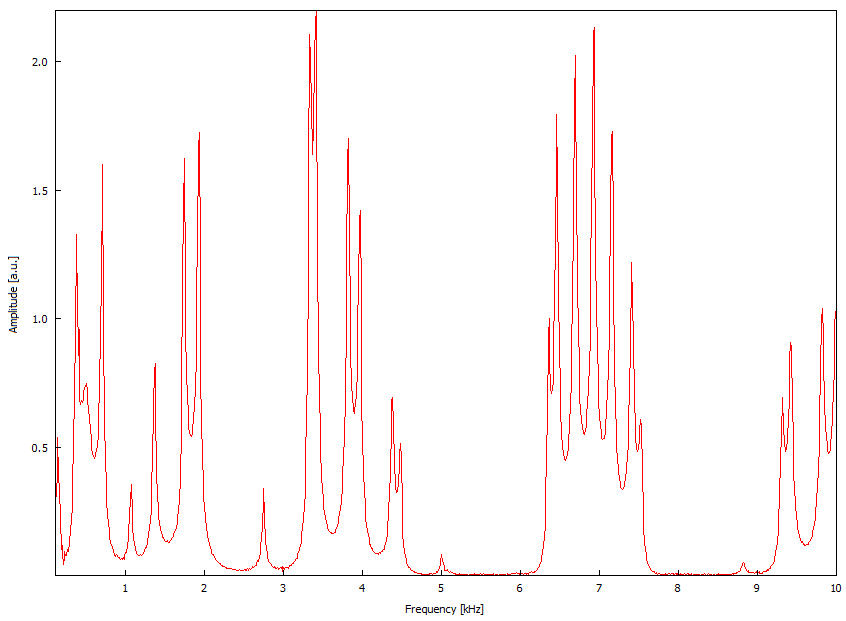
\includegraphics[width=\textwidth]{Bilder/Zylinderketten/unrein_75mm_mitte_doppel_7.png}
    \caption{75mm Fehlstelle}
  \end{subfigure}
  \caption{Resonanzsweeps von Zylinderketten (50mm Zylinder) mit Blenden und einer Fehlstelle}
  \label{fig:zylinder_fehlstellen}
\end{figure}